% Made up for the tikra gallery: chemistry and commutative diagrams inside the drawing, which TikZ
% cannot nest (chemfig and tikz-cd are tikzpictures of their own); mathra sets them as math.
\documentclass[border=0pt]{standalone}
\usepackage{pgfplots}
\usetikzlibrary{backgrounds, arrows.meta}
\definecolor{night}{HTML}{0A0F1F}
\definecolor{ice}{HTML}{7FE3FF}
\definecolor{rose}{HTML}{FF5FA2}
\definecolor{paper}{HTML}{EAF2FF}
\begin{document}
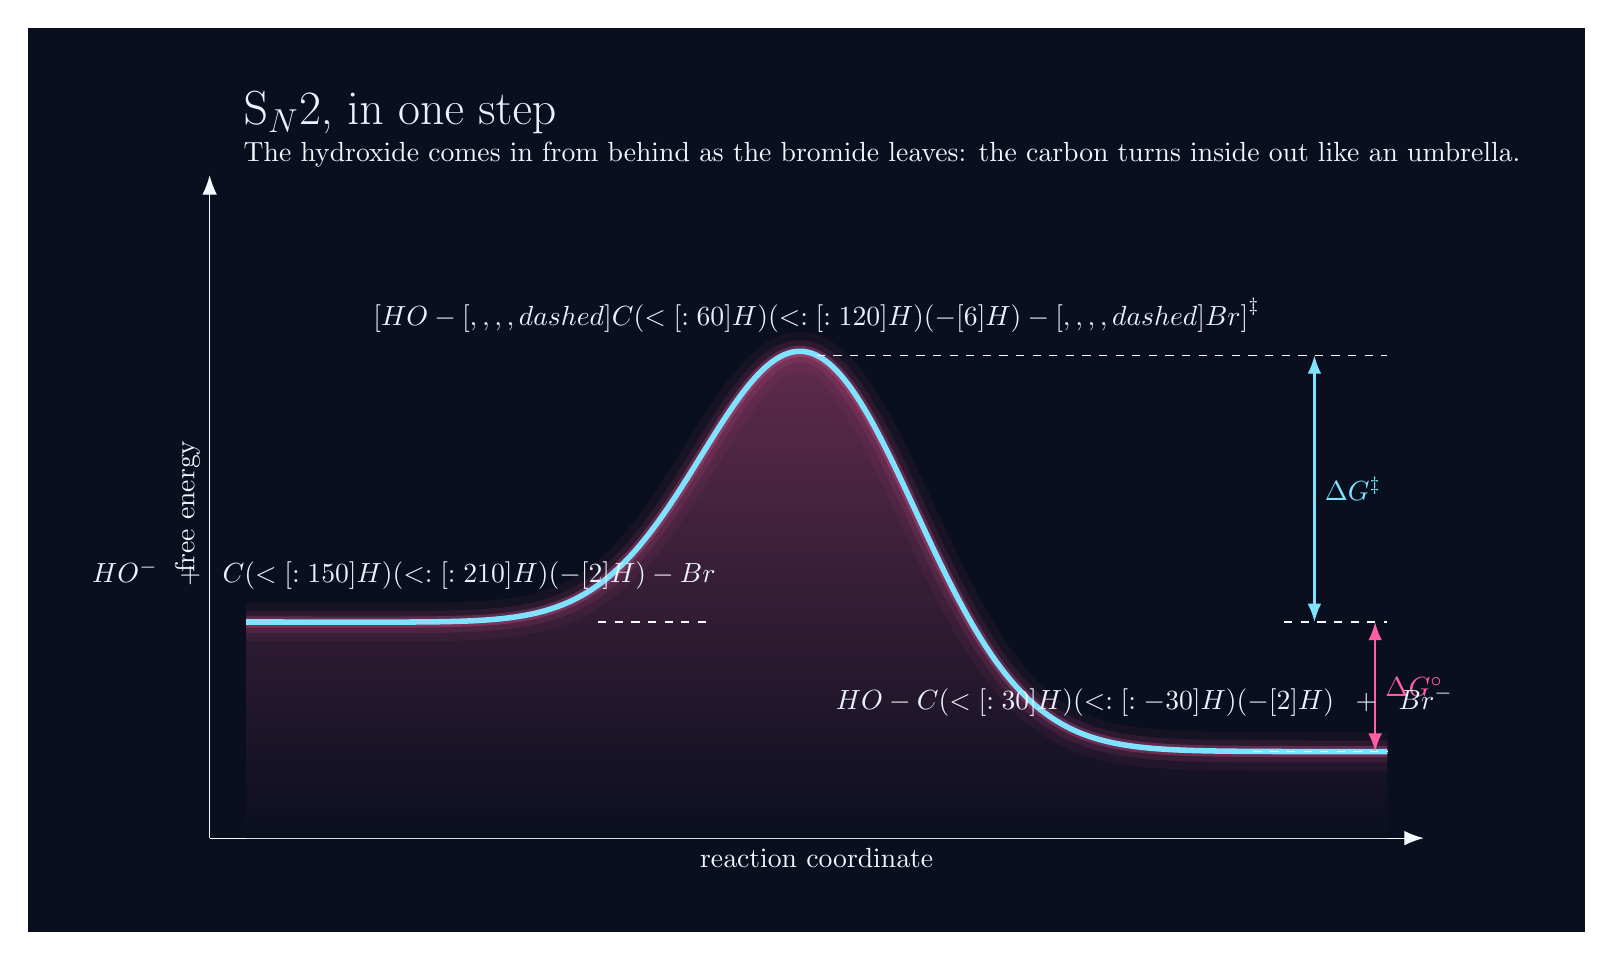
\begin{tikzpicture}[background rectangle/.style={fill=night, draw=none}, show background rectangle, inner frame sep=20pt]
\begin{axis}[width=17cm, height=10cm, clip=false, xmin=0, xmax=10, ymin=-0.75, ymax=1.55,
    axis lines=left, axis line style={paper!45, -{Latex[length=7pt]}}, ticks=none,
    xlabel={reaction coordinate}, ylabel={free energy}, xlabel style={text=paper!60},
    ylabel style={text=paper!60}]
  % the area under the curve, fading down
  \addplot[draw=none, top color=rose!35!night, bottom color=night, domain=0.3:9.7, samples=120] {1.15*exp(-((x-5)/1.25)^2) - 0.45*(1+tanh((x-5)/1.1))/2} -- (axis cs:9.7,-0.75) -- (axis cs:0.3,-0.75) -- cycle;
  % a glow, then the curve
  \addplot[rose, line width=14pt, opacity=0.05, domain=0.3:9.7, samples=120, smooth] {1.15*exp(-((x-5)/1.25)^2) - 0.45*(1+tanh((x-5)/1.1))/2};
  \addplot[rose, line width=8pt, opacity=0.10, domain=0.3:9.7, samples=120, smooth] {1.15*exp(-((x-5)/1.25)^2) - 0.45*(1+tanh((x-5)/1.1))/2};
  \addplot[rose, line width=4pt, opacity=0.25, domain=0.3:9.7, samples=120, smooth] {1.15*exp(-((x-5)/1.25)^2) - 0.45*(1+tanh((x-5)/1.1))/2};
  \addplot[line width=2pt, domain=0.3:9.7, samples=120, smooth, ice] {1.15*exp(-((x-5)/1.25)^2) - 0.45*(1+tanh((x-5)/1.1))/2};
  % levels
  \draw[paper!35, dashed] (axis cs:3.2,0) -- (axis cs:4.1,0);
  \draw[paper!35, dashed] (axis cs:8.85,0) -- (axis cs:9.7,0);
  \draw[paper!35, dashed] (axis cs:5,0.925) -- (axis cs:9.7,0.925);
  \draw[paper!35, dashed] (axis cs:8.6,-0.45) -- (axis cs:9.7,-0.45);
  % energies
  \draw[{Latex}-{Latex}, ice, thick] (axis cs:9.1,0) -- node[right, text=ice] {$\Delta G^{\ddagger}$} (axis cs:9.1,0.925);
  \draw[{Latex}-{Latex}, rose, thick] (axis cs:9.6,0) -- node[right, text=rose] {$\Delta G^{\circ}$} (axis cs:9.6,-0.45);
  % the molecules on the curve
  \node[text=paper, anchor=south] at (axis cs:1.6,0.08)
    {$\chemfig{HO^{-}}\;\;+\;\;\chemfig{C(<[:150]H)(<:[:210]H)(-[2]H)-Br}$};
  \node[text=paper, anchor=south] at (axis cs:5,0.97)
    {$\left[\chemfig{HO-[,,,,dashed]C(<[:60]H)(<:[:120]H)(-[6]H)-[,,,,dashed]Br}\right]^{\ddagger}$};
  \node[text=paper, anchor=south] at (axis cs:7.7,-0.36)
    {$\chemfig{HO-C(<[:30]H)(<:[:-30]H)(-[2]H)}\;\;+\;\;\chemfig{Br^{-}}$};
  \node[anchor=north west, text=paper, font=\LARGE] at (rel axis cs:0.02,1.14) {S$_\text{N}$2, in one step};
  \node[anchor=north west, text=paper!55] at (rel axis cs:0.02,1.065)
    {The hydroxide comes in from behind as the bromide leaves: the carbon turns inside out like an umbrella.};
\end{axis}
\end{tikzpicture}
\end{document}
